\subsection{Numerical Grid}\label{num.sec.grid}
The continuous equations descrining ice physics have to be discretised in order to be solved by a computer (which is inherently finite). This section describes the finite--difference grids employed by the model.
\subsubsection{Horizontal Grid}
The modelled region ($x\in[0,L_x]$, $y\in[0,L_y]$) is discretised using a regular grid so that $x_i=(i-1)\Delta x$ for $i\in[1,N]$ (and similarly for $y_j$). The model uses two staggered horizontal grids in order to improve stability. Both grids use the same grid spacing, $\Delta x$ and $\Delta y$, but are off-set by half a grid (see Fig. \ref{kin.fig.grid}). 
\begin{figure}[htbp]
  \begin{center}
    
\includegraphics{\dir/figs/grid.eps}
    \caption{Horizontal Grid.}
    \label{kin.fig.grid}
  \end{center}
\end{figure}
Quantities calculated on the $(r,s)$--grid are denoted with a tilde, i.e. $\tilde{F}$. Quantities are transformed between grids by averaging over the surrounding nodes, i.e. a quantity in the $(i,j)$--grid becomes in the $(r,s)$ grid:
\begin{subequations}
  \begin{align}
    \tilde{F}_{r,s}&=\tilde{F}_{i+\frac12,j+\frac12}=\frac14(F_{i,j}+F_{i+1,j}+F_{i+1,j+1}+F_{i,j+1})\\
    \intertext{and similarly for the reverse transformation:}
    F_{i,j}&=F_{r-\frac12,s-\frac12}=\frac14(\tilde{F}_{r-1,s-1}+\tilde{F}_{r,s-1}+\tilde{F}_{r,s}+\tilde{F}_{r-1,s})
  \end{align}
\end{subequations}

In general, horizontal velocities and associated quantities like the diffusivity are calculated on the $(r,s)$ grid, ice thickness, temperatures and vertical velocities are calculated on the $(i,j)$--grid.

Horizontal gradients are calculated on the $(r,s)$--grid, i.e. surface gradients are:
\begin{subequations}
\begin{align}
  \left(\frac{\pd s}{\pd x}\right)_{r,s}=\tilde{s}^x_{r,s}&=\frac{s_{i+1,j}-s_{i,j}+s_{i+1,j+1}-s_{i,j+1}}{2\Delta x}\\
  \left(\frac{\pd s}{\pd y}\right)_{r,s}=\tilde{s}^y_{r,s}&=\frac{s_{i,j+1}-s_{i,j}+s_{i+1,j+1}-s_{i+1,j}}{2\Delta y}
\end{align}  
\end{subequations}
Ice thickness gradients, $\tilde{H}^x_{r,s}$ and $\tilde{H}^y_{r,s}$, are formed similarly. Gradients in the $(r,s)$--grid are formed in a similar way, e.g. 
\begin{equation}
  \left(\frac{\pd u}{\pd x}\right)_{i,j}=u^x_{i,j}=\frac{\tilde{u}_{r,s-1}-\tilde{u}_{r-1,s-1}+\tilde{u}_{r,s}-\tilde{u}_{r-1,s}}{2\Delta x}
\end{equation}

\subsubsection{Periodic Boundary Conditions}
The model can be run with horizontal periodic boundary conditions, i.e. the western edge of the modelled region is joined with the eastern edge. Figure \ref{num.fig.grid_ew} illustrates the numeric grid when the model is run in torus mode.

\begin{figure}[htbp]
  \centering
  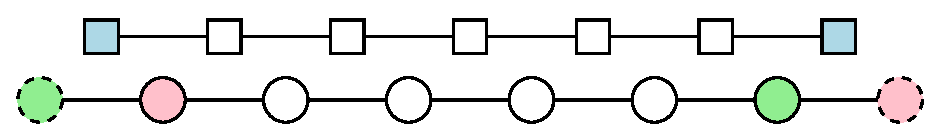
\includegraphics[width=0.9\textwidth]{\dir/figs/grid_ew.eps}
  \caption{A row of the numeric grid when the model is used in torus mode. Circles indicate points in $(i,j)$--grid and squares indicate points in the $(r,s)$--grid. Points with the same colour are logically the same.}
  \label{num.fig.grid_ew}
\end{figure}

These boundary conditions are enforced by exchanging points for the temperature and vertical velocity calculations. The ice thicknesses are calculated explicitly at the ghostpoints.

\subsubsection{$\sigma$--Coordinate System}\label{num.sec.sigma}
The vertical coordinate, $z$, is scaled by the ice thickness analogous to the $s$--coordinate in numerical weather simulations \citep[e.g.][]{Holton1992}. A new vertical coordinate, $\sigma$, is introduced so that the ice surface is at $\sigma=0$ and the ice base at $\sigma=1$ (see Fig. \ref{kin.fig.scale}), i.e.
\begin{equation}
  \label{kin.eq.vertical_scale}
  \sigma=\frac{s-z}{H}.
\end{equation}

\begin{figure}[htbp]
  \begin{center}
    
\includegraphics{\dir/figs/scale.eps}
    \caption[Vertical scaling of the ice sheet model.]{Vertical scaling of the ice sheet model. The vertical axis is scaled to unity. The horizontal coordinates are not changed.}
    \label{kin.fig.scale}
  \end{center}
\end{figure}


The derivatives of a function $f$ in $(x,y,z,t)$ become in the new $(\tilde{x},\tilde{y},\sigma,\tilde{t})$ system:
\begin{subequations}
  \begin{align}
    \frac{\pd f}{\pd x} &= \frac{\pd f}{\pd\tilde{x}}+\frac1H\Delta_{\tilde{x}}\frac{\pd f}{\pd \sigma},\\
    \frac{\pd f}{\pd y} &= \frac{\pd f}{\pd\tilde{y}}+\frac1H\Delta_{\tilde{y}}\frac{\pd f}{\pd \sigma},\\
    \frac{\pd f}{\pd t} &= \frac{\pd f}{\pd\tilde{t}}+\frac1H\Delta_{\tilde{t}}\frac{\pd f}{\pd \sigma},\\
    \frac{\pd f}{\pd z} &= -\frac1H\frac{\pd f}{\pd\sigma},
  \end{align}
\end{subequations}
where  the geometric factors, $\Delta_{\tilde{x}}$, $\Delta_{\tilde{y}}$ and $\Delta_{\tilde{t}}$, are defined by
\begin{subequations}
  \begin{align}
  \Delta_{\tilde{x}}&=\left(\frac{\pd s}{\pd\tilde{x}}-\sigma\frac{\pd H}{\pd\tilde{x}}\right),\\
  \Delta_{\tilde{y}}&=\left(\frac{\pd s}{\pd\tilde{y}}-\sigma\frac{\pd H}{\pd\tilde{y}}\right),\\
  \Delta_{\tilde{t}}&=\left(\frac{\pd s}{\pd\tilde{t}}-\sigma\frac{\pd H}{\pd\tilde{t}}\right).
  \end{align}
\end{subequations}
The integral of $z$ becomes in the $\sigma$--coordinate system:
\begin{equation}
  \int_h^zfdz=-H\int_1^\sigma fd\sigma
\end{equation}

The vertical coordinate is discretised using an irregular grid spacing to reflect the fact that ice flow is more variable at the bottom of the ice column. In the vertical the index $k$ is used. 
